\documentclass[12pt,a4paper,titlepage,twoside,openright]{article}
\usepackage[english]{babel}
\usepackage{ucs} 
\usepackage[utf8x]{inputenc}
\usepackage[usenames,dvipsnames]{xcolor}
\usepackage{tikz,pgfplots}
\usepackage{tkz-tab}
\usepackage{caption}
\usepackage{latexsym}
\usepackage{amssymb}
\usepackage{amsmath}
\usepackage{subcaption} 

\begin{document}
\begin{figure}
    \begin{subfigure}[b]{0.32\textwidth}
        \centering
        \resizebox{\linewidth}{!}{
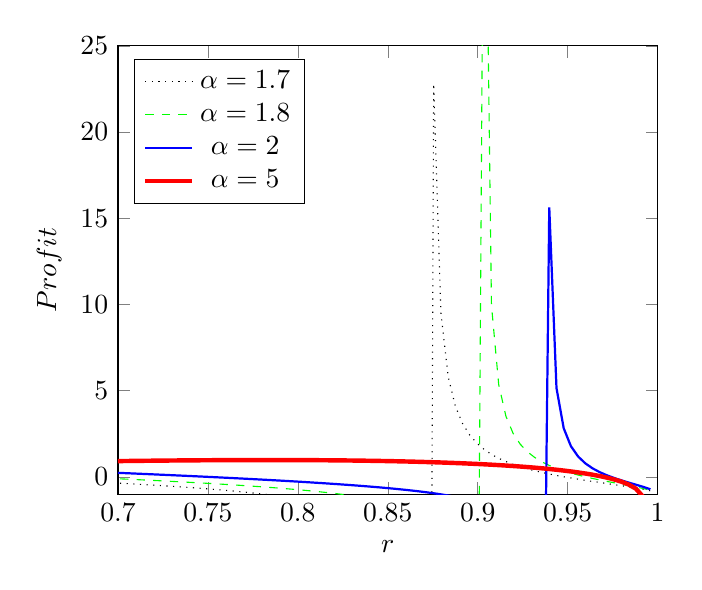
\begin{tikzpicture}
\begin{axis}[legend pos=north west, 
xlabel=$r$,
ylabel={$Profit$}, xmin=0.7,xmax=1,ymin=-1,ymax=25]

\addplot[domain=0:1,samples=250, dotted, black ]{((12*((1.7-1)*sqrt(1-x))-4)*(x+((1.7-1)*sqrt(1-x)))*(x+((1.7-1)*sqrt(1-x))))/((4*((1.7-1)*sqrt(1-x))-1)(4*((1.7-1)*sqrt(1-x))-1))
-((x+((1.7-1)*sqrt(1-x))*(x+((1.7-1)*sqrt(1-x)))/(4*((1.7-1)*sqrt(1-x))-1)*4*((1.7-1)*sqrt(1-x))-1)) } node [pos=0.3, below left]{$\alpha = 1.7$};

\addplot[domain=0:1,samples=250, dashed , green ]{((12*((1.8-1)*sqrt(1-x))-4)*(x+((1.8-1)*sqrt(1-x)))*(x+((1.8-1)*sqrt(1-x))))/((4*((1.8-1)*sqrt(1-x))-1)(4*((1.8-1)*sqrt(1-x))-1))
-((x+((1.8-1)*sqrt(1-x))*(x+((1.8-1)*sqrt(1-x)))/(4*((1.8-1)*sqrt(1-x))-1)*4*((1.8-1)*sqrt(1-x))-1)) } node [pos=0.3, below left]{$\alpha = 1.8$};

\addplot[domain=0:1,samples=250, thick , blue ]{((12*((2-1)*sqrt(1-x))-4)*(x+((2-1)*sqrt(1-x)))*(x+((2-1)*sqrt(1-x))))/((4*((2-1)*sqrt(1-x))-1)(4*((2-1)*sqrt(1-x))-1))
-((x+((2-1)*sqrt(1-x))*(x+((2-1)*sqrt(1-x)))/(4*((2-1)*sqrt(1-x))-1)*4*((2-1)*sqrt(1-x))-1)) } node [pos=0.3, below left]{$\alpha = 2$};

\addplot[domain=0:1,samples=250, ultra thick, red ]{((12*((5-1)*sqrt(1-x))-4)*(x+((5-1)*sqrt(1-x)))*(x+((5-1)*sqrt(1-x))))/((4*((5-1)*sqrt(1-x))-1)(4*((5-1)*sqrt(1-x))-1))
-((x+((5-1)*sqrt(1-x))*(x+((5-1)*sqrt(1-x)))/(4*((5-1)*sqrt(1-x))-1)*4*((5-1)*sqrt(1-x))-1)) } node [pos=0.3, below left]{$\alpha = 5$};
\addlegendentry{$\alpha = 1.7$}
\addlegendentry{$\alpha = 1.8$}
\addlegendentry{$\alpha = 2$}
\addlegendentry{$\alpha = 5$}
\end{axis}
\end{tikzpicture}
        }
        \caption{$\lambda = 0$}
        \label{fig:subfig8}
    \end{subfigure}
    \begin{subfigure}[b]{0.32\textwidth}
    \centering
        \resizebox{\linewidth}{!}{
           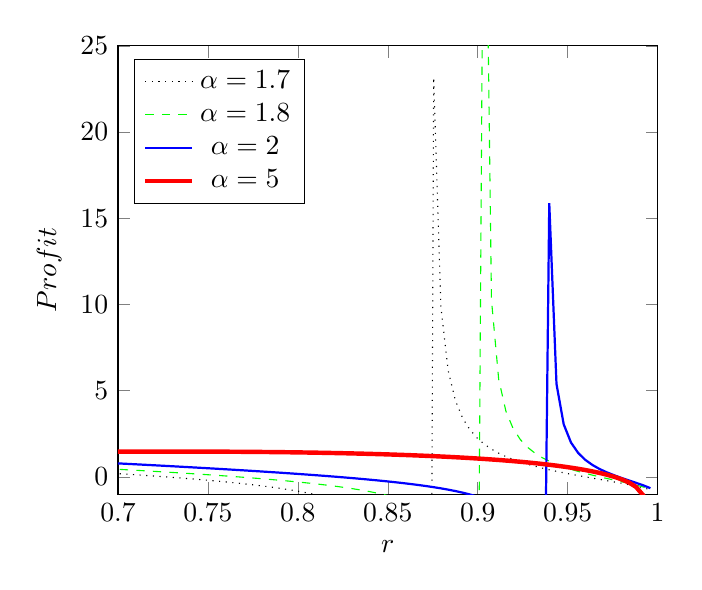
\begin{tikzpicture}
\begin{axis}[ legend pos=north west,
xlabel=$r$,
ylabel={$Profit$}, xmin=0.7,xmax=1,ymin=-1,ymax=25]

\addplot[domain=0:1,samples=250, dotted, black ]{((12*((1.7-1)*sqrt(1-x))-4)*(x+((1.7-1)*sqrt(1-x)))*(x+((1.7-1)*sqrt(1-x))))/((4*((1.7-1)*sqrt(1-x))-1)(4*((1.7-1)*sqrt(1-x))-1))
+1*sqrt(1-x)
-((x+((1.7-1)*sqrt(1-x))*(x+((1.7-1)*sqrt(1-x)))/(4*((1.7-1)*sqrt(1-x))-1)*4*((1.7-1)*sqrt(1-x))-1)) } node [pos=0.3, below left]{$\alpha = 1.7$};

\addplot[domain=0:1,samples=250, dashed, green ]{((12*((1.8-1)*sqrt(1-x))-4)*(x+((1.8-1)*sqrt(1-x)))*(x+((1.8-1)*sqrt(1-x))))/((4*((1.8-1)*sqrt(1-x))-1)(4*((1.8-1)*sqrt(1-x))-1))
+1*sqrt(1-x)
-((x+((1.8-1)*sqrt(1-x))*(x+((1.8-1)*sqrt(1-x)))/(4*((1.8-1)*sqrt(1-x))-1)*4*((1.8-1)*sqrt(1-x))-1)) } node [pos=0.3, below left]{$\alpha = 1.8$};

\addplot[domain=0:1,samples=250, thick, blue ]{((12*((2-1)*sqrt(1-x))-4)*(x+((2-1)*sqrt(1-x)))*(x+((2-1)*sqrt(1-x))))/((4*((2-1)*sqrt(1-x))-1)(4*((2-1)*sqrt(1-x))-1))
+1*sqrt(1-x)
-((x+((2-1)*sqrt(1-x))*(x+((2-1)*sqrt(1-x)))/(4*((2-1)*sqrt(1-x))-1)*4*((2-1)*sqrt(1-x))-1)) } node [pos=0.3, below left]{$\alpha = 2$};

\addplot[domain=0:1,samples=250, ultra thick, red ]{((12*((5-1)*sqrt(1-x))-4)*(x+((5-1)*sqrt(1-x)))*(x+((5-1)*sqrt(1-x))))/((4*((5-1)*sqrt(1-x))-1)(4*((5-1)*sqrt(1-x))-1))
+1*sqrt(1-x)
-((x+((5-1)*sqrt(1-x))*(x+((5-1)*sqrt(1-x)))/(4*((5-1)*sqrt(1-x))-1)*4*((5-1)*sqrt(1-x))-1)) } node [pos=0.3, below left]{$\alpha = 5$};
\addlegendentry{$\alpha = 1.7$}
\addlegendentry{$\alpha = 1.8$}
\addlegendentry{$\alpha = 2$}
\addlegendentry{$\alpha = 5$}
\end{axis}
\end{tikzpicture}
        }
        \caption{$\lambda = 1$}   
        \label{fig:subfig9}
    \end{subfigure}
    \begin{subfigure}[b]{0.32\textwidth}
        \centering
        \resizebox{\linewidth}{!}{
           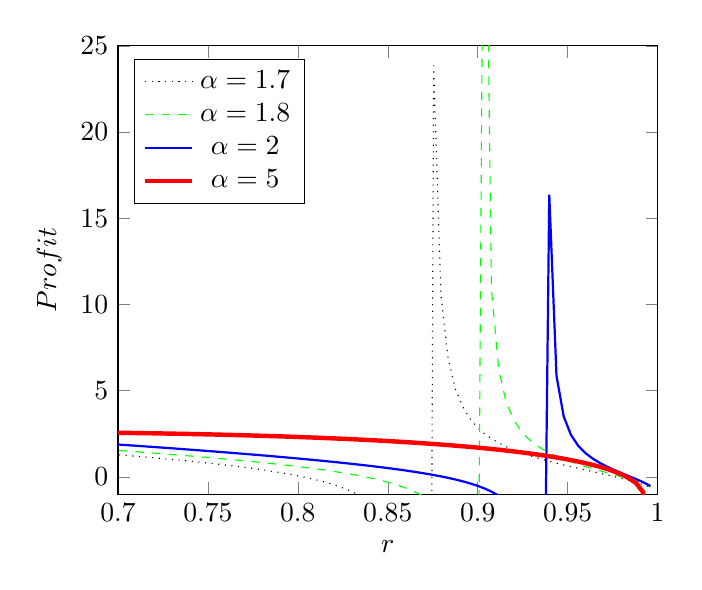
\begin{tikzpicture}
\begin{axis}[ legend pos=north west,
xlabel=$r$,
ylabel={$Profit$}, xmin=0.7,xmax=1,ymin=-1,ymax=25]

\addplot[domain=0:1,samples=250, dotted, black ]{((12*((1.7-1)*sqrt(1-x))-4)*(x+((1.7-1)*sqrt(1-x)))*(x+((1.7-1)*sqrt(1-x))))/((4*((1.7-1)*sqrt(1-x))-1)(4*((1.7-1)*sqrt(1-x))-1))
+3*sqrt(1-x)
-((x+((1.7-1)*sqrt(1-x))*(x+((1.7-1)*sqrt(1-x)))/(4*((1.7-1)*sqrt(1-x))-1)*4*((1.7-1)*sqrt(1-x))-1)) } node [pos=0.3, below left]{$\alpha = 1.7$};

\addplot[domain=0:1,samples=250, dashed, green ]{((12*((1.8-1)*sqrt(1-x))-4)*(x+((1.8-1)*sqrt(1-x)))*(x+((1.8-1)*sqrt(1-x))))/((4*((1.8-1)*sqrt(1-x))-1)(4*((1.8-1)*sqrt(1-x))-1))
+3*sqrt(1-x)
-((x+((1.8-1)*sqrt(1-x))*(x+((1.8-1)*sqrt(1-x)))/(4*((1.8-1)*sqrt(1-x))-1)*4*((1.8-1)*sqrt(1-x))-1)) } node [pos=0.3, below left]{$\alpha = 1.8$};

\addplot[domain=0:1,samples=250, thick, blue ]{((12*((2-1)*sqrt(1-x))-4)*(x+((2-1)*sqrt(1-x)))*(x+((2-1)*sqrt(1-x))))/((4*((2-1)*sqrt(1-x))-1)(4*((2-1)*sqrt(1-x))-1))
+3*sqrt(1-x)
-((x+((2-1)*sqrt(1-x))*(x+((2-1)*sqrt(1-x)))/(4*((2-1)*sqrt(1-x))-1)*4*((2-1)*sqrt(1-x))-1)) } node [pos=0.3, below left]{$\alpha = 2$};

\addplot[domain=0:1,samples=250, ultra thick, red ]{((12*((5-1)*sqrt(1-x))-4)*(x+((5-1)*sqrt(1-x)))*(x+((5-1)*sqrt(1-x))))/((4*((5-1)*sqrt(1-x))-1)(4*((5-1)*sqrt(1-x))-1))
+3*sqrt(1-x)
-((x+((5-1)*sqrt(1-x))*(x+((5-1)*sqrt(1-x)))/(4*((5-1)*sqrt(1-x))-1)*4*((5-1)*sqrt(1-x))-1)) } node [pos=0.3, below left]{$\alpha = 5$};
\addlegendentry{$\alpha = 1.7$}
\addlegendentry{$\alpha = 1.8$}
\addlegendentry{$\alpha = 2$}
\addlegendentry{$\alpha = 5$}
\end{axis}
\end{tikzpicture}
        }
        \caption{$\lambda = 3$}
        \label{fig:subfig10}
    \end{subfigure}
\caption{Profit} 
\label{fig:subfig1.a.4}
\end{figure}

\end{document}